\section{Benchmarking the Implementation Schemes}
\label{bench}
The main problem that we encountered  when implementing cooperative scheduling was saving the context of an execution and resuming from that context. To do this in Java using threads and context switches is simply too expensive and heavily limits the application to the number of native threads that can be created. 

To measure the improvement provided by Java 8 features, we benchmark a
simple example that is illustrated in Fig.~\ref{bench:sf}. In the
example we have one actor containing an  which receives a large
number of messages stored in its queue. This message recursively calls
a function that creates a stack frame after which a message is
sent to a different Actor to run in parallel a function that computes a large number of trigonometric operations . The object is then suspended to await the
result of this function, resulting in the requirement to save the stack frame in order to allow the next message from the queue to run
on the actor.  We varied the total number
of messages in the object's queue to compare performance between a trivial thread based approach and our optimized solution in the Java backend for ABS. 

\begin{figure}
	\label{bench:sf}
	\centering
	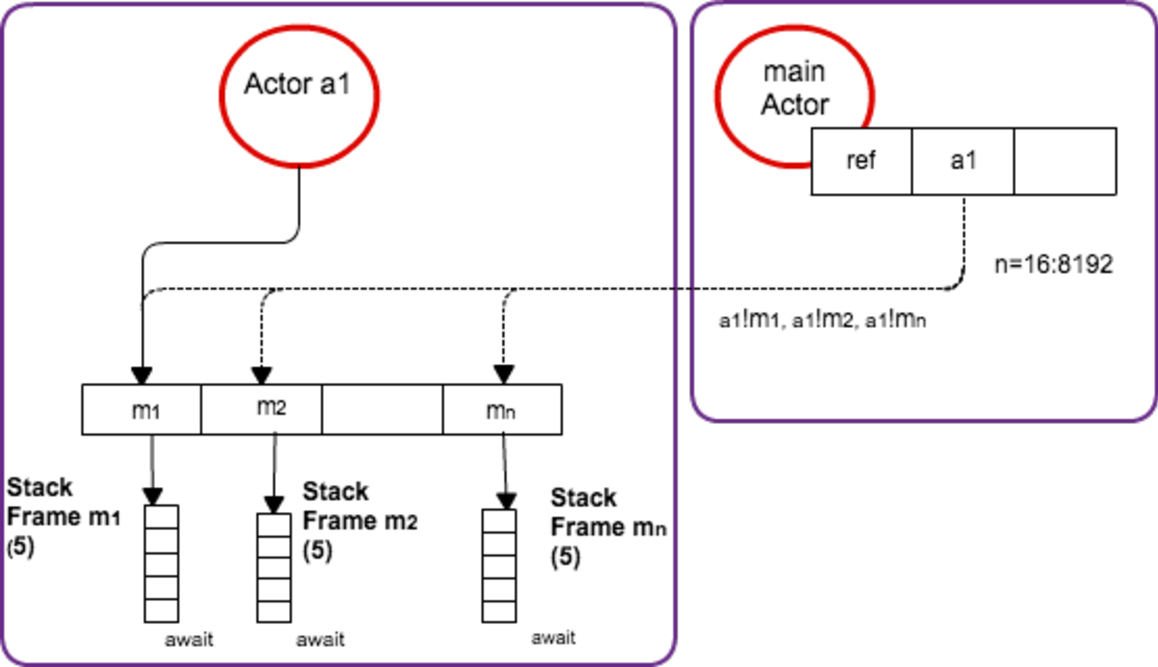
\includegraphics[scale=0.6]{scenario}
	\caption{Cooperative Scheduling Benchmark Scenario}
\end{figure}

\par The results are shown in
Fig.~\ref{bench:jj}. The performance figures presented are for one
actor that is running 16--8192 method invocations, each with a
recursive stack frame of 5 and awaits the
completion of 10000 trigonometric functions before completing. 



\begin{figure}
	\label{bench:jj}
	\centering
	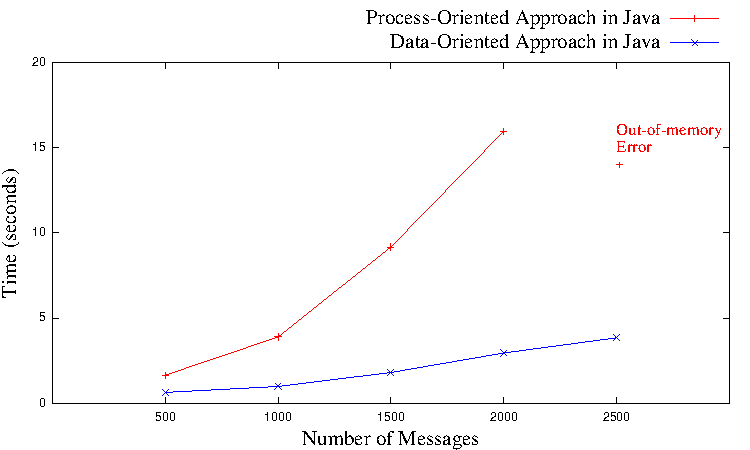
\includegraphics[scale=1]{jaj8.pdf}
	\caption{Performance figures of the two Java implementations for Cooperative Scheduling}
\end{figure}

\par These results do show that our solution mitigates the limitation of heavy native Java threads. However, while our solution is catered towards a widely-used language, it doesn't mean that there aren't other languages that are more suited to implement ABS language concepts efficiently and without these limitations. In Section \ref{scheme} we listed several optimizations that were inferred from out implementation solution. What we want to do is compare this solution to an ABS backend implemented in Erlang that uses the same Thread-based approach but does not suffer from any limitation of native threads. We want to observe if our data-oriented approach can be comparable to Erlang's lightweight threads. The result in Figure \ref{bench:ej} show that our approach fares much better once the number of messages passes 1024. This result also strengthens ABS purpose to provide a programming language for real applications.

\begin{figure}
	\label{bench:ej}
	\centering
	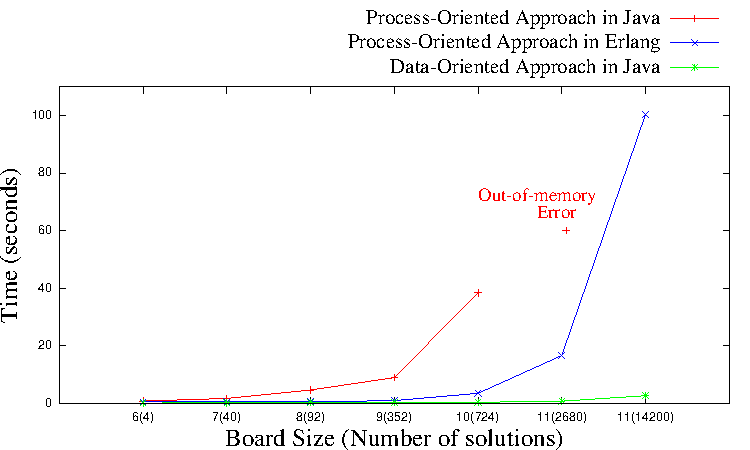
\includegraphics[scale=1]{erlj8.pdf}
	\caption{Performance figures of the Erlang and Java backends for Cooperative Scheduling}
\end{figure}



